\documentclass[tikz,border=0pt,11pt]{standalone}
\usepackage[T1]{fontenc}
\usepackage[utf8]{inputenc}
\usepackage{lmodern,amsmath,amssymb}
\usepackage[swedish]{babel}
\usetikzlibrary{arrows.meta,calc,positioning,decorations.pathmorphing,decorations.pathreplacing,patterns,shadings}
\definecolor{navy}{HTML}{102F40}
\definecolor{teal}{HTML}{147D78}
\definecolor{lightteal}{HTML}{E6F1ED}
\definecolor{gold}{HTML}{B88B3B}
\definecolor{palegold}{HTML}{F7EEDB}
\definecolor{rust}{HTML}{B6533B}
\definecolor{palerust}{HTML}{FAEAE4}
\definecolor{paper}{HTML}{F7F5EE}
\definecolor{muted}{HTML}{5B6D72}
\definecolor{line}{HTML}{D6DED8}
\renewcommand{\familydefault}{\sfdefault}
\newcommand{\atom}[5]{\shade[ball color=#3!70] (#1,#2) circle (#5);\node[text=white,font=\bfseries\small] at (#1,#2){#4};}
\newcommand{\water}[3]{\begin{scope}[shift={(#1,#2)},scale=#3]\draw[navy!45,line width=2pt] (-.3,.22)--(0,0)--(.3,.22);\atom{0}{0}{rust}{O}{.22}\atom{-.3}{.22}{teal}{H}{.15}\atom{.3}{.22}{teal}{H}{.15}\end{scope}}
\newcommand{\panel}[4]{\filldraw[fill=white,draw=line,rounded corners=5pt] (#1,#2) rectangle ++(#3,#4);}
\newcommand{\note}[4]{\node[txt,text width=#3cm] at (#1,#2){#4};}
\tikzset{txt/.style={anchor=north west,align=left,text=navy,font=\small},
 head/.style={anchor=west,text=navy,font=\bfseries\large},
 label/.style={align=center,text=navy,font=\small},
 smalllabel/.style={align=center,text=muted,font=\footnotesize},
 arrow/.style={-{Latex[length=2.5mm,width=1.8mm]},line width=1.2pt,draw=teal},
 goldarrow/.style={-{Latex[length=2.5mm]},line width=1.2pt,draw=gold},
 rustarrow/.style={-{Latex[length=2.5mm]},line width=1.2pt,draw=rust},
 dashedarrow/.style={arrow,dashed},
 badge/.style={fill=lightteal,rounded corners=3pt,text=teal,font=\bfseries\small,inner sep=5pt}}
\begin{document}
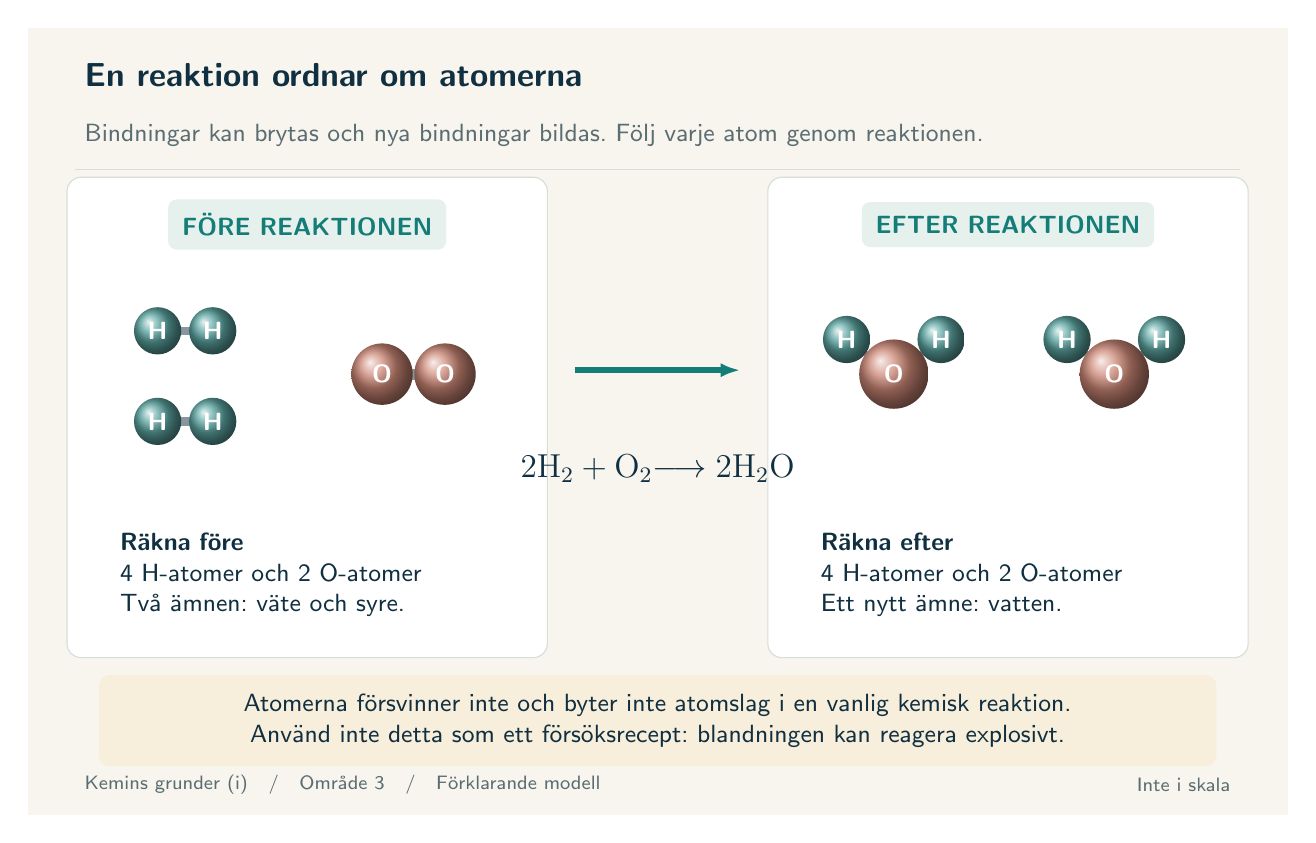
\begin{tikzpicture}[x=1cm,y=1cm]
\path[use as bounding box] (0,0) rectangle (16,10);
\fill[paper] (0,0) rectangle (16,10);
\node[head] at (.6,9.4){En reaktion ordnar om atomerna};
\note{.6}{8.9}{14.8}{\textcolor{muted}{Bindningar kan brytas och nya bindningar bildas. Följ varje atom genom reaktionen.}}
\draw[line] (.6,8.2)--(15.4,8.2);

\panel{.5}{2}{6.1}{6.1}\panel{9.4}{2}{6.1}{6.1}
\node[badge] at (3.55,7.5){FÖRE REAKTIONEN};\node[badge] at (12.45,7.5){EFTER REAKTIONEN};
\foreach \y in {5,6.15}{\draw[navy!50,line width=3pt] (1.65,\y)--(2.35,\y);\atom{1.65}{\y}{teal}{H}{.3}\atom{2.35}{\y}{teal}{H}{.3}}
\draw[navy!50,line width=4pt] (4.5,5.6)--(5.3,5.6);\atom{4.5}{5.6}{rust}{O}{.39}\atom{5.3}{5.6}{rust}{O}{.39}
\water{11}{5.6}{2}\water{13.8}{5.6}{2}
\draw[arrow,line width=2pt] (6.95,5.65)--(9.05,5.65);
\node[label,font=\bfseries\large] at (8,4.4){$2\mathrm{H_2}+\mathrm{O_2}$\par $\longrightarrow 2\mathrm{H_2O}$};
\note{1.05}{3.7}{5.0}{\textbf{Räkna före}\par 4 H-atomer och 2 O-atomer\par Två ämnen: väte och syre.}
\note{9.95}{3.7}{5.0}{\textbf{Räkna efter}\par 4 H-atomer och 2 O-atomer\par Ett nytt ämne: vatten.}
\node[label,fill=palegold,rounded corners=4pt,inner sep=7pt,text width=13.7cm] at (8,1.2){Atomerna försvinner inte och byter inte atomslag i en vanlig kemisk reaktion. Använd inte detta som ett försöksrecept: blandningen kan reagera explosivt.};\node[anchor=west,text=muted,font=\scriptsize] at (.6,.38){Kemins grunder (i)\quad /\quad Område 3\quad /\quad Förklarande modell};
\node[anchor=east,text=muted,font=\scriptsize] at (15.4,.38){Inte i skala};
\end{tikzpicture}\end{document}
